\section{Abstract Interpretation}\label{sec:abstrint}

Abstract interpretation is among the most well known methods of static
analysis of programs. First introduced by Patrick and Radhia Cousot
in~\cite{patrickradhia:one, patrickradhia:two} and consists in a
sound-by-construction method to infer program properties given a model
of their behavior. The general idea is that we can approximate the
semantics of a program with monotonic functions over ordered sets
(usually \emph{complete lattices}). To do so we usually first
introduce \emph{Abstract Domains} that capture some essential aspect
of program execution while ignoring the details of the computation,
which would make the analysis computationally infeasible.  This
analysis however carries the issue of completeness, which is closely
related to the issue of choosing the best abstract domain to decide
program correctness without raising false alarms. Achieving
completeness in analysis is often desirable, but it can lead to the
problem of undecidability. This means that even though we strive for
the most accurate analysis of a program, such as through its
interpreter, we can't guarantee that the process will always
terminate.  The technique per-se is a concept which is around since
the '70s, hence an extensive amount of literature has been
produced. For a brief history of the technique,
see~\cite{ranzato:history}.

The main source of this chapter comes from the notes on abstract
interpretation in~\cite{mine:course}.

\subsection{General concepts}\label{subsec:abstrgeneral}

Abstract interpretation heavily relies on order theory, which we
introduced in Section~\ref{sec:ordertheory}, and builds on top of
it. The core idea is that we use an \emph{abstract domain} as an
approximation of the \emph{concrete domain}, in such a way that
abstract computations are \emph{sound} with respect to the concrete
ones. The minimal structure that we will require both in the abstract
and the concrete domains is a partial order that models the amount of
information each instruction carries with respect to the program
execution. Thus, the concrete domain is a partially ordered set
\(\tuple{C, \leq}\) (e.g.\ integers powersets) and the abstract domain
is another partially ordered set \(\tuple{A, \sqsubseteq}\) (e.g.\
intervals). The minimal amount of connection between these two worlds
is a \emph{concretization} functions
\begin{definition}[Concretization]
  A concretization function
  \(\gamma : \tuple{A , \sqsubseteq} \to \tuple{C, \leq}\) is a
  \emph{monotonic} function, i.e.
  \begin{equation*}
    \forall a,a' \in A \quad a \sqsubseteq a' \Rightarrow \gamma(a) \leq \gamma(a')
  \end{equation*}
\end{definition}

Trough concretization we have a first notion of \emph{soundness}

\begin{definition}[Soundness]\label{def:soundness}
  \(a \in A\) is a \emph{sound} abstraction of \(c\in C\) iff
  \(c \leq \gamma(a)\).
\end{definition}

While monotonic concretizations are sufficient to reason about
soundness, more structure is useful to design a sound and
\emph{accurate} analyzer. The standard abstract interpretation
framework from~\cite{patrickradhia:one} also assumes the existence of
some monotonic \emph{abstraction function}
\({\abstr : \tuple{C, \leq} \to \tuple{A, \sqsubseteq}}\), such that
\(\tuple{\abstr, C, A, \concr}\) forms a Galois connection:

\begin{definition}[Galois connection]\label{def:galoiscon}
  Given two partially ordered sets
  \(\tuple{C, \leq}, \tuple{A, \sqsubseteq}\), the tuple
  \(\tuple{\abstr, C, A, \concr}\) is a Galois connection if
  \begin{itemize}
  \item \(A,C\) are complete lattices;
  \item \(\abstr : \tuple{C, \leq} \to \tuple{A, \sqsubseteq}\) and
    \(\concr : \tuple{A, \sqsubseteq} \to \tuple{C, \leq}\) are monotonic;
  \item for all \(a\in A, c\in C\),
    \begin{equation}\label{eq:conn}
      c \leq \concr(a) \iff \abstr(c) \sqsubseteq a.
    \end{equation}
  \end{itemize}

  We denote \(\tuple{\abstr, C, A, \concr}\) as
  \({\tuple{C, \leq} \galois{\abstr}{\concr} \tuple{A, \sqsubseteq}}\).
\end{definition}

\begin{figure}
  \centering
  \usetikzlibrary{arrows.meta}
  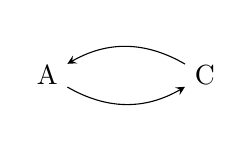
\begin{tikzpicture}[->, >=stealth]
    % Nodes
    \node (A) at (0,0) {A};
    \node (C) at (2,0) {C};
    
    % Arrows
    \path
    (C) edge[bend right=30] node[above]{$\abstr$} (A)
    (A) edge[bend right=30] node[below]{$\concr$} (C);
  \end{tikzpicture}
  \caption{Galois connection between an abstract domain \(A\) and a
    concrete domain \(C\)}\label{fig:galois}
\end{figure}

Usually though we use an alternative characterization of Galois
Connections, which is easier to prove:

\begin{theorem}\label{th:alternate}
  \(\tuple{C, \leq} \galois{\abstr}{\concr} \tuple{A, \sqsubseteq}\)
  is a Galois connection iff the function pair
  \(\tuple{\abstr,\concr}\) satisfies all the following properties:
  \begin{enumerate}[label=(\arabic*)]
  \item \(\abstr, \concr\) are monotonic;
  \item \(\forall c \in C \quad c \leq \concr(\abstr(c))\) i.e.,
    \(\concr \circ \abstr\) is extensive;
  \item \(\forall a \in A \quad \abstr(\concr(a)) \sqsubseteq a\),
    i.e., \(\abstr \circ \concr\) is reductive.
  \end{enumerate}
\end{theorem}

\begin{proof}
  Assume that \(\tuple{\abstr,\concr}\) satisfies~\eqref{eq:conn},
  then we want to prove that the properties of
  Theorem~\ref{th:alternate} hold.
  \begin{enumerate}[label=(\arabic*)]
  \item\label{proof:one} Applying~\eqref{eq:conn} with
    \(a \defin \abstr(c)\) we get
    \begin{equation}
      c \leq \concr(\abstr(c))
    \end{equation}
    i.e., \(\concr \circ\abstr\) is extensive, which is our first
    thesis.
  \item\label{proof:two} Applying~\eqref{eq:conn} with
    \(c \defin\concr(a)\) we get
    \begin{equation}
      \abstr(\concr(a)) \sqsubseteq a
    \end{equation}
    i.e., \(\abstr\circ\concr\) is reductive, which is our second
    thesis.
  \item By~\ref{proof:one} \(\forall c, c'\in C\) it holds that
    \(c \leq c' \Rightarrow c \leq \concr(\abstr(c'))\). Hence, we can
    apply again~\eqref{eq:conn} with \(a \defin \abstr(c')\) and get
    that \(\abstr(c) \sqsubseteq \abstr(c')\), i.e., \(\abstr\) is
    monotonic.
  \item By~\ref{proof:two} \(\forall a, a'\in C\) it holds that
    \(a \sqsubseteq a' \Rightarrow \abstr(\concr(a)) \sqsubseteq
    a\). Hence, we can apply~\eqref{eq:conn} with
    \(c \defin \concr(a)\) and get that
    \(\concr(a)\leq\concr(a')\), i.e., \(\concr\) is
    monotonic.
  \end{enumerate}

  Assume conversely that the four properties hold. Then we want to
  prove that~\eqref{eq:conn} holds.
  \begin{description}
  \item[(\(\Rightarrow\))] First assume that \(c \leq
    \concr(a)\). Then \(\abstr(c) \sqsubseteq \abstr(\concr(a))\) by
    monotonicity of \(\abstr\) and \(\abstr(\concr(a)) \sqsubseteq a\)
    by reductivity, hence \(\abstr(c) \sqsubseteq a\).
  \item[(\(\Leftarrow\))] Likewise, assume that
    \(\abstr(c) \sqsubseteq a\). Then
    \(\concr(\abstr(c)) \leq \concr(a)\) by monotonicity of \(\concr\)
    and \(c \leq \concr(\abstr(c))\) by extensivity, hence
    \(c \leq \concr(a)\).
  \end{description}
\end{proof}

Galois connections carry with them some well known properties, that
are useful to state best correct approximations (bca) and to prove the
soundness by construction of the analyzer:

\begin{theorem}[Galois connection properties]\label{th:galoisprop}
  Given a Galois connection
  \(\tuple{C,\leq} \galois{\abstr}{\concr} \tuple{A, \sqsubseteq}\) we
  have:
  \begin{enumerate}
  \item \(\concr \circ \abstr \circ \concr = \concr\) and
    \(\abstr \circ \concr \circ \abstr = \abstr\);
  \item \(\abstr \circ \concr\) and \(\concr \circ \abstr\) are
    idempotent;
  \item\label{prop:three} \(\forall c \in C\)
    \(\abstr(c) = \sqcap \{a \mid c \leq \concr(a)\}\);
  \item \(\forall a \in A\)
    \(\concr(a) = \vee \{ c \mid \abstr(c) \sqsubseteq a \}\);
  \item\label{prop:five} \(\abstr\) maps concrete lubs to abstract lubs:
    \begin{equation*}
      \forall X \subseteq C \quad \exists \vee X \Rightarrow \abstr(\vee X) = \sqcup \{\abstr(x) \mid x \in X\}
    \end{equation*}
  \item \(\concr\) maps abstract glbs to concrete glbs:
    \begin{equation*}
      \forall X \subseteq A \quad \exists \sqcap X \Rightarrow \concr(\sqcap X) = \wedge \{\concr(x) \mid x \in X\}
    \end{equation*}
  \end{enumerate}
\end{theorem}

Theorem~\ref{th:galoisprop} states two important properties of Galois
connections: \emph{soundness} and \emph{optimality}. Recall that
\(c \leq \concr(a)\) means by Definition~\ref{def:soundness} that
\(a\) is a \emph{sound} approximation of \(c\). Then, given
\(c \in C\) recall that \(c \leq \concr(\abstr(c))\), which means that
\(\abstr(c)\) is a sound abstraction of \(c\). Finally,
Property~\ref{prop:three} states that \(\abstr(c)\) is the best (i.e.,
smallest) sound abstraction of \(c\), i.e., the \emph{optimal}
abstraction.

Additionally, from the theorem we can derive the
following corollary:

\begin{corollary}[Best abstraction]\label{co:bestabstr}
  If we have a Galois connection \(\tuple{\abstr, C, A, \concr}\),
  then \(\forall c \in C, \abstr(c)\) is the \emph{best abstraction}
  of \(c\), i.e., the smallest abstract element which is a sound
  abstraction of \(c\).
\end{corollary}

In general we saw that for a Galois connection \(\concr \conc \abstr\)
is idempotent, and generally not the identity function, as abstracting
looses precision. Concretizing however, should not loose precision, so
we could expect \(\abstr \circ \concr\) to be the identity
function. When this is the case, we have a \emph{Galois insertion}:

\begin{definition}[Galois Insertion]\label{def:insertion}
  A Galois
  connection \(\tuple{C, \leq} \galois{\abstr}{\concr} \tuple{A,
    \sqsubseteq}\) is a \emph{Galois insertion} if one of the
  following, equivalent properties hold:
  \begin{enumerate}
  \item \(\abstr\) is surjective: \(\forall a \in A\)
    \(\exists c \in C \mid \abstr(c) = a\);
  \item \(\concr\) is injective: \(\forall a, a'\in A\)
    \(\concr(a) = \concr(a') \Rightarrow a = a'\);
  \item \(\abstr \circ \concr\) is the identity function.
  \end{enumerate}
  We denote Galois insertions as
  \(\tuple{C, \leq} \galoiS{\abstr}{\concr} \tuple{A, \sqsubseteq}\).
\end{definition}

Nexr, we can show that given a Galois connection and by doing a
\emph{point-wise lifting} of the values in the concrete and abstract
domain, we get another galois connection. This will later be useful in
Chapter~\ref{chap:abstractdomains} to lift proofs from a domain to its
point-wilse lifting.

\begin{theorem}\label{th:pointwiseconn}
  Given a Galois connection
  \(\tuple{C, \leq} \galois{\abstr}{\concr} \tuple{A, \sqsubseteq}\)
  we can derive a new Galois connection with the \emph{point wise
    lifting}, i.e.
  \(\tuple{S\to C, \ovdot{\leq}} \galois{\dot\abstr}{\ovdot{\concr}}
  \tuple{S\to A, \ovdot{\sqsubseteq}}\) where
  \begin{align*}
    f \dot\leq f' & \defin \forall s \in S \quad f(s) \leq f'(s)\\
    f \dot\sqsubseteq f' & \defin \forall s \in S \quad f(s) \sqsubseteq f'(s)\\
    \dot\abstr(f) & \defin \lambda s \in S . \abstr(f(s)) \\
    \dot\concr(f) & \defin \lambda s \in S . \concr(f(s)) \\
  \end{align*}
  and \(S\) is an arbitrary set.
\end{theorem}

\begin{proof}
  \begin{align*}
    \dot\abstr(c) \ovdot\sqsubseteq a & \iff \forall x\in S \quad \abstr(c)(x) \sqsubseteq a(x) & \text{by definition} \\
                                      & \iff \forall x\in S \quad c(x) \leq a(x) & \text{by~\eqref{eq:conn}} \\
                                      & \iff c \ovdot\leq \dot\concr(a) & \text{by definition}
  \end{align*}
\end{proof}

from this, we can derive the following
\begin{theorem}\label{th:liftingins}
  if
  \(\tuple{C, \leq} \galoiS{\abstr}{\concr} \tuple{A, \sqsubseteq}\)
  is a Galois insertion, then its point-wise lifting is again a Galois
  insertion:
  \begin{equation*}
    \tuple{S \to C, \ovdot\leq} \galoiS{\dot\abstr}{\dot\concr} \tuple{S\to A, \ovdot\sqsubseteq}
  \end{equation*}
\end{theorem}

\begin{proof}
  By Th.~\ref{th:pointwiseconn} it holds that
  \(\tuple{S \to C, \ovdot\leq} \galois{\dot\abstr}{\dot\concr}
  \tuple{S\to A, \ovdot\sqsubseteq}\). What we have to prove is that
  \(\dot\abstr \circ \dot\concr = \id\) kowing that
  \(\abstr \circ \concr = \id\).

  \begin{align*}
    (\dot\abstr \circ \dot\concr)(f) & = \dot\abstr(\lambda s\in S . \concr(f(s))) & \text{by definition} \\
                                     & = \lambda s\in S . (\abstr \circ \concr)(f(s)) & \text{by definition} \\
                                     & = \lambda s\in S . \id(f(s)) & \text{by hypothesis} \\
                                     & = f & \text{by definition}
  \end{align*}
  hence \(\dot\abstr \circ \dot\concr = \id\), which means
  \(\tuple{S \to C, \ovdot\leq} \galoiS{\dot\abstr}{\dot\concr}
  \tuple{S\to A, \ovdot\sqsubseteq}\).
\end{proof}

In this context we also need a way of ensuring abstract operations are
sound (and occasionally) correct. Even by only using the
concretization map and no Galois connection, the notion of sound and
correct abstraction carries naturally from domain elements to domain
operators:

\begin{definition}[Sound and correct operator abstraction]
  Let \(\concr : \tuple{A \sqsubseteq} \to \tuple{C, \leq}\) be a
  concretization map from an abstract domain
  \(\tuple{A, \sqsubseteq}\) to a concrete domain \(\tuple{C, \leq}\),
  \(f : C \to C\) be a concrete operator and \(g : A \to A\) an
  abstract operator.
  \begin{enumerate}
  \item \(g\) is a \emph{sound abstraction} of \(f\) if
    \(\forall a \in A \quad f(\concr(a)) \leq \concr(g(a))\);
  \item \(g\) is a \emph{correct abstraction} of \(f\) if
    \(f \circ \concr = \concr \circ g\).
  \end{enumerate}
\end{definition}

Notice that a correct abstraction is always sound.  Another remarkable
thing of Galois connections, is that along with this notion we can
introduce the notion of \emph{Best correct approximation}:

\begin{definition}[Best correct approximation (bca)]
  Given a Galois connection \(\tuple{\abstr, C, A, \concr}\) and a
  concrete operator \(f : C \to C\), the \emph{best abstraction} of
  \(f\) is given by \(\abstr \conc f \conc \concr\).
\end{definition}

It is imperative to prioritize the modular and composable nature of
our abstractions. As elaborated in subsequent chapters, the semantics
of a program typically emerge from the composition of atomic semantic
functions drawn from a finite library representing fundamental
language operations. This framework lends itself well to a modular
abstraction scheme, where abstract operators are designed exclusively
for this foundational set of operations. By adhering to the same
principles governing concrete semantics, these abstract operators can
be composed effectively. This is facilitated by the inherent
composability and accuracy of sound abstractions:

\begin{theorem}[Operator composition]\label{th:opcomp}
  Let \(f, f' : C \to C\) be concrete operators and \(g, g' A \to A\)
  abstract operators. The following properties hold:
  \begin{enumerate}[label=(\arabic*)]
  \item if \(g, g'\) are \emph{sound abstractions} of \(f\) and \(f'\)
    respectively and \(f\) is monotonic, then \(g \circ g'\) is a
    sound abstraction of \(f \circ f'\);
  \item if \(g, g'\) are correct abstractions of \(f\) and \(f'\)
    respectively then \(g \circ g'\) is a correct abstraction of
    \(f \circ f'\).
  \end{enumerate}
\end{theorem}

\begin{proof}
  We proceed to prove the two properties in order:
  \begin{enumerate}[label=(\arabic*)]
  \item \(g'\) is a sound abstraction of \(f'\), hence
    \begin{align*}
      \forall a \in A \quad (f'\circ \concr)(a) & \leq (\concr \circ g') (a) \\
      (f \circ f' \circ \concr)(a) & \leq (f \circ \concr \circ g')(a) & \text{by monotonicity of } f \\
      (f \circ f' \circ \concr)(a) & \leq (f \circ \concr \circ g')(a) \leq (\concr \circ g \circ g')(a) & \text{by monotonicity of } g
    \end{align*}
  \item since both \({f \circ \concr = \concr \circ g}\) and
    \({f' \circ \concr = \concr \circ g'}\) it holds that
    \begin{equation*}
      f \circ f' \circ \concr =  f \circ \concr \circ g' = \concr \circ g \circ g'
    \end{equation*}
  \end{enumerate}
\end{proof}

\subsection{Fixpoint approximations}\label{subsec:fixpointapprox}
Critical parts of program semantics are defined trough the idea of
least fixpoints \(\lfp f\) of some monotonic function or continuous
operator \(f : C \to C\) over the concrete domain
\(\tuple{C,\leq}\). In order to abstract the computation of \(\lfp f\)
in the abstract domain \(\tuple{A,\sqsubseteq}\) the natural idea is
to start with a sound abstraction \(g : A \to A\) of \(f\). Then there
are many ways of approximate the fixpoint computation trough the use
of \(g\). We mention two, in order to see what its main problems are.

\begin{description}
\item[Kleene fixpoint.] A first idea is to mimic the fixpoint
  computation with \(g\) instead of \(f\). For instance by relying on
  the constructive definition of \(\lfp f\) as the limit of an
  iteration sequence from Kleene's Theorem~\ref{th:fixpoint}:
  \begin{equation*}
    \lfp(f) = \sqcup\{f^i(\bot) \mid i \in \n\} \sqsubseteq \sqcup\{g^i(\bot) \mid i \in \n\} = \lfp(g)
  \end{equation*}
  
\item[Tarski fixpoint.] Tarski fixpoint is instead based on the Tarski
  characterization of the fixpoint:
  \begin{equation}\label{eq:tarski}
    \lfp(f) = \sqcap \{x \in C \mid f(x) \sqsubseteq x\}
  \end{equation}
  i.e., the least fixpoint of a monotonic function \(f\) over a
  complete lattice \(f\) is the greatest lower bound of the
  postfixpoints.  The observation is that any abstract postfixpoint of
  a sound abstract rapresents, trough \(\concr\), a concrete fixpoint
  (by Theorem~\ref{th:galoisprop}). The theorem however does not state
  how to compute a postfixpoint of \(g\) in the abstract, but is
  nonetheless useful as it allows us to provide a sound answer (a
  post-fixpoint) even with abstract fixpoints are difficult to compute
  (as for infinite ascending chains) or non-existstent at all.
\end{description}

As mentioned before, in order to solve the convergence problem in
abstract domains,Patrick and Radhia Cousot in~\cite{patrickradhia:one}
prposed to use Tarski's characterization to provide post fixpoint of
infinite ascending chains, introducing a binary operator: the
\emph{widening} operator \(\widen\).

\begin{definition}[Widening operator]\label{def:widen}
  A binary operator \(\widen : A \times X \to A\) is a \emph{widening
    operator} in an abstract domain \(\tuple{A, \sqsubseteq}\) if
  \begin{enumerate}
  \item it computes upper bounds:
    \begin{equation*}
      \forall x, y \in A \quad x \sqsubseteq x \widen y \; \land \; y \sqsubseteq x \widen y;
    \end{equation*}
  \item\label{widen:prop1} it enforces convergence: for any sequence
    \({\{y^i\}}_{i\in\n}\) in \(A\), the sequence
    \({\{z^i\}}_{i\in\n}\) computed as
    \begin{align*}
      z^0 & \defin y^0 \\
      z^{i+1} & \defin z^i \narrowi y^{i+1}
    \end{align*}
    stabilizes in finite time: \(\exists k \geq 0 \mid x^{k+1} = x^k\).
  \end{enumerate}
\end{definition}

With the widening operator we enforce the termination of a sound
abstract analyzer for the computation of upper bounds:

\begin{theorem}\label{th:convergence}
  Let \(f\) be a monotonic operator in a complete concrete lattice and
  \(g\) a sonud abstraction of \(f\). Then the following iteration
  \begin{align*}
    x^0 & \defin \bot \\
    x^{i+1} & \defin x^i \widen g(x^i)
  \end{align*}
  converges in finite time, and its limit \(x\) is a sound abstraction
  of the least fixpoint \(\lfp(f)\), i.e., \(\lfp(f) \leq \concr(x)\).
\end{theorem}

\begin{proof}
  Convergence is ensured by Property~\ref{widen:prop1} of
  Definition~\ref{def:widen}, while the soundness is because of
  Equation~\eqref{eq:tarski} given that, when encountering a stable
  value \(x^{i+1} = x^i\), then
  \(f(x^i) \sqsubseteq x^i \widen f(x^i) = x^{i+1}\), i.e., \(x^i\) is
  an abstract postfixpoint.
\end{proof}

Where the first point states that \(\narrowi\) refines its left
argument while bringing a sound approximation, and the second point
enforces termination.

